\documentclass[a4paper]{article}
\usepackage[utf8]{inputenc}
\usepackage[russian,english]{babel}
\usepackage[T2A]{fontenc}
\usepackage[left=10mm, top=20mm, right=18mm, bottom=15mm, footskip=10mm]{geometry}
\usepackage{indentfirst}
\usepackage{circuitikz}
\usepackage{tikz}
\usepackage{amsmath,amssymb}
\usepackage[italicdiff]{physics}
\usepackage{graphicx}
\usetikzlibrary{patterns}
% \usetikzlibrary{circuits.ee.IEC}
\usepackage{pgfplots}
\pgfplotsset{compat=1.18}
\graphicspath{{images/}}
\DeclareGraphicsExtensions{.pdf,.png,.jpg}
\usepackage{wrapfig}
\usepackage{float}
\usepackage{subcaption}
\usepackage{enumitem}
\usepackage{caption}
\captionsetup[figure]{name=Рисунок}
\captionsetup[table]{name=Таблица}

\title{\underline{Занятие по резонансам в колебательном контуре}}
\author{Воронин Денис, Дрожжин Никита Б04-407}

\begin{document}

\maketitle

\section{Элементы колебательного контура}
\subsection{c) Конденсатор ёмкостью C (может зависеть от частоты,амплитуды,иметь активное сопротивление).}

\section*{1. Вступление (Идеальная модель)}

Идеальный конденсатор — устройство, которое накапливает заряд и обладает ёмкостью \(C\). Его основное свойство — чистое реактивное сопротивление, обратно пропорциональное частоте:
\[
X_C = \frac{1}{\omega C} = \frac{1}{2\pi f C}
\]
где \(\omega = 2\pi f\) — круговая частота.\par
Реактивное сопротивление (X) не рассеивает энергию в виде тепла. Оно лишь временно накапливает и отдает энергию обратно в цепь. Конденсатор делает это в виде энергии электрического поля.

Проще говоря, реактивное сопротивление — это "сопротивление" конденсатора изменению напряжения.\par
На постоянном токе (\(f = 0\)) \(X_C \to \infty\) (разрыв цепи), а с ростом частоты сопротивление стремится к нулю.

\textbf{ Применение и значение}

Благодаря своим свойствам конденсаторы используются для:
\begin{itemize}
    \item \textbf{Разделения цепей постоянного и переменного тока}: Постоянная составляющая не пройдёт, а переменный сигнал (например, звук) — пройдёт.
    \item \textbf{Фильтрации частот}: Вместе с резисторами или катушками индуктивности они образуют фильтры (высокочастотные, низкочастотные, полосовые). Это основа работы всей аудиоаппаратуры, радиоприёмников и т.д.
    \item \textbf{Создания фазосдвигающих цепей} (используется, например, в пусковых схемах электродвигателей).
    \item \textbf{Стабилизации питания в цепях} (сглаживающие конденсаторы).
\end{itemize}

\textbf{Итог простыми словами:}

Реактивное сопротивление конденсатора ($X_C$) — это мера того, как конденсатор <<противится>> прохождению переменного тока, но не за счёт превращения энергии в тепло, а за счёт её накопления и возврата. Его величина зависит от двух вещей: чем \textbf{БОЛЬШЕ} ёмкость и чем \textbf{ВЫШЕ} частота тока, тем \textbf{ЛЕГЧЕ} току пройти через конденсатор (тем меньше $X_C$). Это свойство делает конденсатор незаменимым элементом для управления сигналами разной частоты в электронных схемах.

\section*{2. Реальная модель и её элементы}

В реальности любой конденсатор — сложное устройство. Его поведение описывает \textbf{схема замещения}:

\begin{figure}[h]
    \centering
    \begin{circuitikz}[european]
        % Идеальный конденсатор
        \draw (0,0) to[C, l=\(C\), o-o] (2,0);
        \node at (1,-0.7) {а) Идеальная модель};
        
        % Реальная модель (последовательная)
        \begin{scope}[xshift=4cm]
            \draw (0,0) to[R, l=\(R_s\) (ESR), o-] (1.5,0) to[L, l=\(L_s\) (ESL), -] (3,0) to[C, l=\(C\), -o] (4.5,0);
            \node at (2.25,-0.7) {б) Реальная модель (RLC-замещение)};
        \end{scope}
    \end{circuitikz}
    \label{fig:shemy}
\end{figure}

Основные неидеальности:
\begin{enumerate}
    \item \textbf{Активное последовательное сопротивление (ESR)} —(Суммарное активное сопротивление, "встроенное" в конденсатор. Оно ведёт себя так, как будто последовательно с идеальной ёмкостью включён резистор.) сопротивление выводов, обкладок и диэлектрика. Вызывает нагрев и потери энергии.
    \item \textbf{Паразитная индуктивность (ESL)} — (Паразитная индуктивность, "встроенная" в конструкцию конденсатора. Величина обычно очень небольшая (единицы-десятки наногенри), но её влияние становится определяющим на высоких частотах.) индуктивность выводов и обкладок, критична на высоких частотах.
    \item \textbf{Сопротивление утечки (R\_утечки)} — моделирует ток утечки через диэлектрик (обычно параллельно \(C\), не показано).
\end{enumerate}

Полный комплексный импеданс последовательной модели:
\[
\dot{Z} = R_s + j\omega L_s + \frac{1}{j\omega C} = R_s + j\left(\omega L_s - \frac{1}{\omega C}\right)
\]
Модуль импеданса:
\[
|Z| = \sqrt{R_s^2 + \left(\omega L_s - \frac{1}{\omega C}\right)^2}
\]

Из формулы виден эффект \textbf{резонанса}: на частоте \(f_{\text{рез}} = \frac{1}{2\pi\sqrt{L_s C}}\) мнимые части компенсируются, импеданс минимален и равен \(R_s\). Выше этой частоты конденсатор ведёт себя как индуктивность.

\begin{figure}[h!]
	\centering
	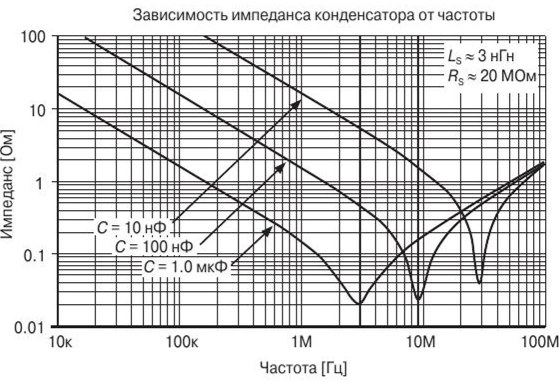
\includegraphics[width=10cm]{27.PNG}
	\caption{Зависимость емкости от частоты}
	\label{fig:Holl2}
\end{figure}

\section*{3. Зависимость от частоты и амплитуды}

\begin{itemize}
    \item \textbf{От частоты:} Зависимость \emph{кажущейся} ёмкости от частоты обусловлена свойствами диэлектрика (медленные виды поляризации не успевают реагировать) и влиянием \(L_s\), \(R_s\). На графике (рис. \ref{fig:impedance}) видно отклонение реального импеданса от идеального \(X_C\).

    \item \textbf{От амплитуды (напряжения):} Для диэлектриков с нелинейной проницаемостью (керамика типа X7R, Z5U) ёмкость зависит от постоянного смещения \(U_0\):
    \[
    C(U_0) \approx C_0 \cdot (1 - \alpha U_0^2)
    \]
    где \(\alpha > 0\) — коэффициент нелинейности. При большом переменном сигнале это вызывает нелинейные искажения.
\end{itemize}

\section*{4. Мера потерь: тангенс угла потерь}

Для оценки качества используют \textbf{тангенс угла потерь} \(\tan \delta\), где \(\delta\) — угол между векторами полного тока и реактивного тока в конденсаторе (или дополнение до \(90^\circ\) фазового угла \(\varphi\) импеданса: \(\delta = 90^\circ - \varphi\)).

\begin{figure}[h]
    \centering
    \begin{tikzpicture}[scale=1.2]
        \draw[->] (0,0) -- (4,0) node[below] {\(I \cdot R_s\) (активная составляющая)};
        \draw[->] (0,0) -- (0,3) node[left] {\(I \cdot X\) (реактивная составляющая)};
        \draw[->, thick] (0,0) -- (3.5, 1.5) node[above right] {\(\dot{U} = I \cdot \dot{Z}\)};
        \draw (0.7,0) arc (0:23:0.7) node[midway, right] {\(\varphi\)};
        \draw (23:1.5) arc (23:90:1.5) node[midway, above right] {\(\delta\)};
        \draw[dashed] (3.5,1.5) -- (3.5,0);
        \draw[dashed] (3.5,1.5) -- (0,1.5);
    \end{tikzpicture}
    \caption{Векторная диаграмма для последовательной модели}
    \label{fig:vector}
\end{figure}

Для последовательной модели:
\[
\tan \delta = \frac{R_s}{|X_C|} = \omega C R_s
\]

Для параллельной модели (ёмкость \(C\) и сопротивление утечки \(R_p\)):
\[
\tan \delta \approx \frac{1}{\omega C R_p}
\]

Чем меньше \(\tan \delta\), тем ближе конденсатор к идеальному.

\section*{5. Заключение}

Реальный конденсатор — это комплексный частотно-зависимый импеданс с активными потерями и паразитной индуктивностью. Его ёмкость может нелинейно зависеть от амплитуды приложенного напряжения. Учёт этих факторов (через ESR, ESL, \(\tan \delta\), \(C(U)\)) критически важен для проектирования современных электронных схем, особенно силовых, высокочастотных и прецизионных.

\section{Схема колебательного контура и основные уравнения}
\subsection{c.	Уравнения для описания процессов в последовательном колебательном контуре из идеальных элементов.}

\subsection*{1. Схема и основные элементы}

Последовательный колебательный контур состоит из трёх идеальных элементов, соединённых последовательно:

\begin{center}
\begin{circuitikz}[european]
    \draw (0,0) to[sinusoidal voltage source, v<=$e(t)$] (0,2) -- (2,2) 
          to[inductor, l=$L$, i=$i(t)$] (4,2) 
          to[capacitor, l=$C$, v=$u_C$] (6,2) -- (8,2)
          to[resistor, l=$R$, v=$u_R$] (8,0) -- (0,0);
    \draw[thin, <-] (1,1.5) arc (60:120:0.5) node[left] {$u_L$};
\end{circuitikz}
\end{center}

\begin{itemize}
    \item $L$ — индуктивность катушки [Гн]
    \item $C$ — ёмкость конденсатора [Ф]
    \item $R$ — сопротивление резистора [Ом]
    \item $e(t)$ — внешняя ЭДС (в автономном контуре $e(t)=0$)
\end{itemize}

\subsection*{2. Вывод дифференциального уравнения}

По второму закону Кирхгофа сумма напряжений в контуре равна ЭДС:
\[
u_L + u_R + u_C = e(t)
\]
Используем соотношения для идеальных элементов:
\[
u_L = L \frac{di}{dt}, \quad u_R = Ri, \quad i = C \frac{du_C}{dt}
\]
Ток через конденсатор: $i = C \frac{du_C}{dt}$. Подставляем в уравнение:
\[
L \frac{d}{dt}\left(C \frac{du_C}{dt}\right) + R C \frac{du_C}{dt} + u_C = e(t)
\]
Получаем дифференциальное уравнение второго порядка относительно напряжения $u_C(t)$:
\[
\boxed{LC \frac{d^2 u_C}{dt^2} + RC \frac{du_C}{dt} + u_C = e(t)}
\]

Аналогично, выражая через заряд $q(t)$ на конденсаторе ($q = Cu_C$, $i = dq/dt$):
\[
\boxed{L \frac{d^2 q}{dt^2} + R \frac{dq}{dt} + \frac{1}{C} q = e(t)}
\]

Для автономного контура ($e(t)=0$) уравнение становится однородным:
\[
L \frac{d^2 q}{dt^2} + R \frac{dq}{dt} + \frac{1}{C} q = 0
\]

\subsection*{3. Решение для свободных колебаний ($e(t)=0$)}

Введём параметры:
\[
\alpha = \frac{R}{2L} \quad \text{(коэффициент затухания)}, \quad \omega_0 = \frac{1}{\sqrt{LC}} \quad \text{(собственная частота)}
\]
Уравнение принимает вид:
\[
\frac{d^2 q}{dt^2} + 2\alpha \frac{dq}{dt} + \omega_0^2 q = 0
\]

Характеристическое уравнение:
\[
\lambda^2 + 2\alpha \lambda + \omega_0^2 = 0
\]
Корни:
\[
\lambda_{1,2} = -\alpha \pm \sqrt{\alpha^2 - \omega_0^2}
\]

В зависимости от соотношения $\alpha$ и $\omega_0$ получаем три режима:

\begin{enumerate}
    \item \textbf{Колебательный режим} ($\alpha < \omega_0$): \\
    $\omega = \sqrt{\omega_0^2 - \alpha^2}$ — частота затухающих колебаний. \\
    Решение: 
    \[
    q(t) = A_0 e^{-\alpha t} \cos(\omega t + \varphi_0)
    \]
    \item \textbf{Критический режим} ($\alpha = \omega_0$): \\
    Решение:
    \[
    q(t) = (A_1 + A_2 t) e^{-\alpha t}
    \]
    \item \textbf{Апериодический режим} ($\alpha > \omega_0$): \\
    $\beta = \sqrt{\alpha^2 - \omega_0^2}$ \\
    Решение:
    \[
    q(t) = e^{-\alpha t} \left( B_1 e^{\beta t} + B_2 e^{-\beta t} \right)
    \]
\end{enumerate}

\subsection*{4. График затухающих колебаний ($\alpha < \omega_0$)}

\begin{center}
\begin{tikzpicture}
    \begin{axis}[
        width=0.8\textwidth,
        height=0.4\textwidth,
        xlabel={Время $t$, с},
        ylabel={Заряд $q(t)$},
        grid=both,
        axis lines=middle,
        xmin=0, xmax=10,
        ymin=-1.2, ymax=1.2,
        samples=200,
        domain=0:10,
        legend pos=north east,
    ]
    \addplot[blue, thick] {exp(-0.3*x)*cos(deg(2*pi*x))};
    \addplot[red, dashed, thick] {exp(-0.3*x)};
    \addplot[red, dashed, thick] {-exp(-0.3*x)};
    \legend{$q(t)=A_0 e^{-\alpha t} \cos(\omega t + \varphi_0)$, $A_0 e^{-\alpha t}$, $-A_0 e^{-\alpha t}$};
    \end{axis}
\end{tikzpicture}
\end{center}

\subsection*{5. Добротность контура}

Важной характеристикой является \textbf{добротность} $Q$:
\[
Q = \frac{\omega_0}{2\alpha} = \frac{1}{R} \sqrt{\frac{L}{C}}
\]
Для высокодобротных контуров ($Q \gg 1$) затухание мало, и колебания продолжаются долго.

\subsection*{6. Вынужденные колебания}

При гармонической ЭДС $e(t) = E_m \cos(\Omega t)$ устанавливаются вынужденные колебания с частотой $\Omega$. Амплитуда зависит от соотношения $\Omega$ и $\omega_0$, достигая максимума при резонансе ($\Omega = \omega_0$).

\subsection*{Заключение}

Таким образом, процессы в последовательном колебательном контуре описываются линейным дифференциальным уравнением второго порядка. Его решение позволяет определить режимы работы контура (колебательный, критический, апериодический) и важные характеристики, такие как частота и добротность, что является основой для анализа и проектирования радиотехнических устройств.


\section{Измерения в колебательном контуре}
\subsection{a.	Измерение напряжения}

\section*{Введение}
Колебательный контур — основа радиотехники и электроники. Его способность избирательно усиливать сигналы на определённой частоте (резонансной) делает его ключевым элементом в приёмниках, генераторах и фильтрах. \textbf{Измерение напряжения} на элементах контура позволяет определить его основные параметры: резонансную частоту, добротность, полосу пропускания.

\section*{1. Уравнение колебаний и его решение}
Рассмотрим простейший последовательный $RLC$-контур. При свободных колебаниях (после воздействия внешнего импульса) напряжение на конденсаторе $u_C(t)$ описывается дифференциальным уравнением:
\[
LC\frac{d^2u_C}{dt^2} + RC\frac{du_C}{dt} + u_C = 0
\]
Решение этого уравнения при малых потерях ($R^2 < \frac{4L}{C}$) имеет вид \textbf{затухающих гармонических колебаний}:
\begin{equation}
\boxed{u_C(t) = U_0 e^{-\delta t} \cos(\omega t + \varphi_0)}
\end{equation}
где:
\begin{itemize}
    \item $U_0$ — начальная амплитуда,
    \item $\delta = \frac{R}{2L}$ — коэффициент затухания,
    \item $\omega = \sqrt{\omega_0^2 - \delta^2}$ — циклическая частота свободных колебаний,
    \item $\omega_0 = \frac{1}{\sqrt{LC}}$ — собственная (резонансная) частота контура.
\end{itemize}

\begin{figure}[h!]
\centering
\begin{tikzpicture}[scale=1.2]
    % Оси
    \draw[->] (0,0) -- (6,0) node[right] {$t$};
    \draw[->] (0,-2.2) -- (0,2.2) node[above] {$u_C(t)$};
    \draw (0,0) node[below left] {0};
    % Огибающая
    \draw[dashed, blue, thick, domain=0:5.5, samples=100] plot (\x, {1.8*exp(-0.35*\x)});
    \draw[dashed, blue, thick, domain=0:5.5, samples=100] plot (\x, {-1.8*exp(-0.35*\x)});
    % Колебания
    \draw[red, thick, domain=0:5.5, samples=250] plot (\x, {1.8*exp(-0.35*\x)*cos(6*(\x+0.15) r)});
    % Подписи
    \draw[<->] (1.57,0.8) -- (3.14,0.8) node[midway,above] {$T=\frac{2\pi}{\omega}$};
    \draw[<->] (0.5,1.9) -- (0.5,0.5) node[midway,right] {$U_0 e^{-\delta t}$};
\end{tikzpicture}
\caption{График затухающих колебаний напряжения на конденсаторе $u_C(t)$}
\end{figure}

\section*{2. Методы измерения напряжения}
\subsection*{2.1. Прямое измерение (осциллограф)}
Самый наглядный способ — подключение осциллографического щупа параллельно элементу контура (конденсатору или катушке). Мы непосредственно видим форму $u(t)$, как на рис. 1, и можем измерить:
\begin{itemize}
    \item Амплитуду (в моменты $t=0$, $t=T$ и т.д.).
    \item Период $T$, а значит и частоту $\omega = 2\pi / T$.
    \item \textbf{Декремент затухания} $\Lambda = \ln\left|\frac{u(t)}{u(t+T)}\right| = \delta T$. Отсюда можно найти добротность: $Q = \frac{\pi}{\Lambda}$.
\end{itemize}
\textbf{Важно!} Щуп осциллографа вносит в контур дополнительную ёмкость и сопротивление, искажая измерения.

\subsection*{2.2. Косвенное измерение (резонансная кривая)}
Чаще на практике измеряют не свободные, а \textbf{вынужденные колебания}. Подают на контур от генератора синусоидальный сигнал частоты $f$ и измеряют напряжение на конденсаторе вольтметром (или осциллографом).

При изменении частоты получают \textbf{резонансную кривую} $U_C(f)$. Максимум этой кривой соответствует резонансной частоте $f_0 = \frac{1}{2\pi\sqrt{LC}}$. По \textbf{полосе пропускания} $\Delta f = f_2 - f_1$ (уровень $0.707$ от максимума) находят добротность:
\begin{equation}
\boxed{Q = \frac{f_0}{\Delta f}}
\end{equation}

\section*{Заключение}
Измерение напряжения в колебательном контуре — не просто снятие показаний. Это \textbf{метод диагностики} контура, позволяющий определить его фундаментальные характеристики: частоту, добротность, затухание. Правильный выбор метода измерения (прямая визуализация или снятие АЧХ) и учёт влияния измерительных приборов — залог точности в радиотехнических расчётах и настройке устройств.

\section{Импедансы}
\subsection{b.	Импеданс идеальной катушки индуктивности, импеданс реальной катушки}

\subsection*{Введение}
Импеданс ($Z$) — это комплексное сопротивление элемента цепи переменному току, учитывающее как диссипативные (омические), так и реактивные (индуктивные, емкостные) свойства. Он измеряется в Омах и является обобщением закона Ома для цепей переменного тока:
\[
\dot{U} = \dot{I} \cdot Z
\]
где $\dot{U}$ и $\dot{I}$ — комплексные амплитуды напряжения и тока.

\subsection*{Импеданс идеальной катушки индуктивности}
Идеальная катушка обладает только индуктивностью $L$ и не имеет активного сопротивления. Для такой катушки справедливо известное соотношение: напряжение опережает ток на угол $\frac{\pi}{2}$ (90$^\circ$).

\begin{wrapfigure}{r}{0.3\textwidth}
    \centering
    \begin{tikzpicture}
        % Рисуем индуктивность в виде зигзага
        \draw (0,0) -- (0.5,0);
        \draw (0.5,0) -- (0.5,0.5);
        \draw (0.5,0.5) -- (1,0.5);
        \draw (1,0.5) -- (1,0);
        \draw (1,0) -- (1.5,0);
        \draw (1.5,0) -- (1.5,0.5);
        \draw (1.5,0.5) -- (2,0.5);
        \draw (2,0.5) -- (2,0);
        \draw (2,0) -- (2.5,0);
        % Выводы
        \draw (-0.5,0) -- (0,0);
        \draw (2.5,0) -- (3,0);
        % Обозначение
        \node at (1.25, -0.5) {$L$};
        \draw (-0.5,0) node[circ] {};
        \draw (3,0) node[circ] {};
    \end{tikzpicture}
    \caption{Идеальная катушка}
\end{wrapfigure}

Импеданс идеальной катушки является чисто мнимым и рассчитывается по формуле:
\[
Z_L = j \omega L
\]
\textbf{Краткий вывод:}
Из закона электромагнитной индукции: $u_L = L \frac{di}{dt}$.
Пусть ток изменяется по гармоническому закону: $i(t) = I_m \sin(\omega t)$.
Тогда:
\[
u_L = L \frac{d}{dt}(I_m \sin(\omega t)) = \omega L I_m \cos(\omega t) = \omega L I_m \sin(\omega t + \frac{\pi}{2})
\]
Сравнивая амплитуды, получаем $U_m = I_m \cdot \omega L$. В комплексной форме сдвиг на $+\frac{\pi}{2}$ даёт множитель $j = e^{j\pi/2}$. Следовательно, $Z_L = \frac{\dot{U}_m}{\dot{I}_m} = j\omega L$.

Модуль импеданса $|Z_L| = X_L = \omega L$ называется \textbf{индуктивным сопротивлением}. Оно линейно растёт с увеличением частоты $\omega$.

\subsection*{Импеданс реальной катушки}
Реальная катушка, помимо индуктивности $L$, обладает:
\begin{itemize}
    \item Активным сопротивлением провода обмотки $R_\text{пр}$.
    \item Паразитной межвитковой ёмкостью $C_\text{пар}$.
\end{itemize}

\begin{figure}[h!]
    \centering
    \begin{tikzpicture}[every node/.style={font=\small}]
        % Рисуем эквивалентную схему
        % Источник переменного тока
        \draw (0,0) to [short, o-] (0.5,0);
        % Резистор
        \draw (1,0) to [resistor, l=$R_\text{пр}$] (3,0);
        % Катушка индуктивности (упрощённое обозначение)
        \draw (3,0) to [inductor, l=$L$] (5,0);
        % Паразитная ёмкость (рисуем параллельно)
        \draw (1,0) -- (1,-1.5) to [capacitor, l=$C_\text{пар}$] (5,-1.5) -- (5,0);
        % Замыкаем цепь
        \draw (5,0) -- (5.5,0) to [short, -o] (6,0);
        \draw (0,0) to [open, v=$\sim$] (0,-1.5) -- (6,-1.5) to [short, -o] (6,0);
        % Точки для обозначения
        \draw (0,0) node[ocirc] {};
        \draw (6,0) node[ocirc] {};
    \end{tikzpicture}
    \caption{Эквивалентная схема реальной катушки}
\end{figure}

На низких и средних частотах влиянием ёмкости часто можно пренебречь. Тогда схема упрощается до последовательного соединения $R_\text{пр}$ и $L$.

Импеданс такой катушки становится комплексным:
\[
Z_\text{реал} = R_\text{пр} + j\omega L
\]

\vspace{2mm}
Его основные характеристики:
\begin{itemize}
    \item \textbf{Модуль:} $|Z_\text{реал}| = \sqrt{R_\text{пр}^2 + (\omega L)^2}$
    \item \textbf{Фазовый сдвиг:} $\varphi = \arctg\left(\frac{\omega L}{R_\text{пр}}\right)$
    \item \textbf{Добротность:} $Q = \frac{\omega L}{R_\text{пр}} = \tg \varphi$ — важный параметр, характеризующий «качество» катушки.
\end{itemize}

На \textbf{высоких частотах} паразитная ёмкость $C_\text{пар}$ шунтирует катушку. Полный импеданс параллельного $LC$-контура (с потерями $R_\text{пр}$) имеет сложную зависимость от частоты и может носить резонансный характер.

\subsection*{Сравнение и вывод}
\begin{center}
    \begin{tabular}{|l|l|l|}
        \hline
        \textbf{Параметр} & \textbf{Идеальная катушка} & \textbf{Реальная катушка (на НЧ)} \\
        \hline
        Схема & Чистая $L$ & Последовательные $R_\text{пр}$ и $L$ \\
        \hline
        Импеданс, $Z$ & $j\omega L$ & $R_\text{пр} + j\omega L$ \\
        \hline
        Напряжение и ток & Сдвиг ровно на 90$^\circ$ & Сдвиг $< 90^\circ$ ($\varphi = \arctg(\omega L/R_\text{пр})$) \\
        \hline
        Поведение на постоянном токе ($\omega=0$) & Короткое замыкание ($Z=0$) & Резистор ($Z = R_\text{пр}$) \\
        \hline
    \end{tabular}
\end{center}

Таким образом, импеданс реальной катушки всегда имеет как активную, так и реактивную составляющую. Идеальная модель справедлива только при $R_\text{пр} \ll \omega L$, то есть на достаточно высоких частотах для катушки с высокой добротностью. Учёт реального импеданса критически важен при проектировании фильтров, колебательных контуров и других высокочастотных устройств.

\end{document}